\chapter{Podobné obrázky}


Jednou ze služeb, které výsledná aplikace poskytuje, je vyhledávání podobných obrázků. Uživatel rozhraní najde pomocí textových dotazů nějaké ilustrační obrázky a má možnost u každého z nalezených obrázků získat obrázky vizuálně podobné. Tato kapitola pojednává o tvorbě backendové služby, která vyhledávání podobných obrázků umožňuje.

Vstupními daty je soubor s vektory pro každý obrázek datasetu Profimedie. Vektor má $4 096$ složek s reálnými nezápornými čísly. Vektory jsou vizuální deskriptory obrázků. Tyto deskriptory byly vygenerovány pomocí software Caffe\cite{caffe} a jsou jsou odezvami předposlední vrstvy hluboké konvoluční neuronové sítě natrénované pro klasifikaci obrázků z datasetu Profimedie do 1000 kategorii.

Mějme obrázek $I_1$ s deskriptorem $D_1$ a obrázek $I_2$ s deskriptorem $D_2$. Míru podobnosti obrázků $Similarity$ pak můžeme definovat jako

\begin{equation}
  Similarity(I_1, I_2) = \sum_{i=1}^{4096} |D_1[i]-D_2[i]|
\end{equation}

V praxi se dají výsledky této míry klasifikovat zhruba do 3 kategorií. Tyto vypozorované kategorie popisuje tabulka \ref{fig:simtypes}. Ukázky jednotlivých kategorií podobných obrázků poskytuje obrázek \ref{fig:simexamples}. Rozdělení na 3 kategorie podobnosti podle míry $Similarity$ je pouze přibližné. Nelze například zaručit, že obrázek, který by některý uživatel mohl uznačit za podobný, nebude mít míru $Similarity$ vyšší než $1 500$.

\begin{figure}[h]
\label{fig:simtypes}
\centering
\begin{tabular}{ | c | r |}
  \hline
     Kategorie & $Similarity$\\
  \hline
  \hline
    téměř shodné & $0 - 500$ \\
  \hline
    podobné & $500 - 1500$ \\
  \hline
    nepodobné & $> 1500$ \\
\hline
\end{tabular}

  \caption{Kategorie podobnosti obrázků podle $Similarity$.}
\end{figure}

\begin{figure}[h]
  \centering
  \includegraphics[width=150mm]{similar_images.eps}
  \caption{Dvojice obrázků s různou kategorií podobnosti.}
  \label{fig:simexamples}
\end{figure}

Otázkou zůstává, které výsledky uživatel očekává jako výsledky vyhledávání podobných obrázků. Pravděpodobně nechce získat obrázky z kategorie \uv{nepodobné}. Pak je otázkou, jestli uživatel chce jako výsledek získat obrázky z kategorie \uv{téměř shodné}. V korpusu je spousta podmnožin obrázků, které byly vyfoceny v rámci jedné série. Často se liší jen malou změnou úhlu fotky, nebo jen kompresí uloženého obrázku. Pokud bychom vraceli obrázky seřezené podle $Similarity$, uživatelé u takovýchto podmnožit nedostanou příliš rozmanité obrázky. Vracet obrázky seřazené podle $Similarity$ tedy nemusí být vždy vhodné, náhodné pořadí obrázků z kategorií \uv{téměř shodné} a \uv{podobné} může uživatel chápat jako lepší výsledek. Tato úvaha umožňuje použít algoritmy, které nevrací obrázky seřazené podle $Similarity$, ale jsou výrazně rychlejší.


\section{Bootstrap implementace}

První implementace nahrála všechny deskriptory do databáze Elasticsearch. V Elasticsearch lze implementovat vyhledávání pomocí vlastní porovnávací funkce. Jako porovnávací funkce tedy zvolíme funkci $Similarity$. Bohužel přes některé menší optimalizace algoritmu se vyhledávání nepodařilo implementovat příliš efektivně, takže fungovalo v přijatelném čase pouze pro pár tisíc deskriptorů. Naše aplikace ovšem potřebuje pracovat s více než dvaceti miliony deskriptorů. Šly by použít další optimalizace a sharding databáze na více strojů, aby algoritmus fungoval efektivněji i na větším množství dat. To by ovšem bylo příliš drahé a navíc se objevily jiné možnosti řešení.


\section{Předgenerování výsledků}

Efektivnější variantou je ke každému obrázku vygenerovat nějaké množství podobných obrázků předem. Služba která by vracela podobné obrázky by pouze vrátila položku z databáze a neprováděla žádný výpočet. Tato služba by tak byla velmi rychlá a nenáročná na zdroje. Jako problém se ovšem ukázalo právě předgenerování obrázků. Přes snahu o co nejrychlejší implementaci v jazyce go s použitím více vláken a optimalizačních heuristik, by vygenerování podobných obrázků pro každý z 20 milionů obrázků v datasetu Profimedie trvalo na běžném počítači několik týdnů.

\section{Geohash}
Další pokus o implementaci vyhledávání podobných obrázků se inspiruje algoritmem Geohash\cite{geohash}. Algoritmus Geohash byl vyvinut v rámci služby geohash.org a jedná se o způsob zakódování prostorových dat. Jeho hlavním využitím je efektivní vyhledávání bodů (určených zeměpisnými souřadnicemi) v oblasti (na mapě). Algoritmus Geohash využívá i Google, nebo databáze Elasticsearch.

Zjednodušení algoritmu Geohash popíšeme na jednotkové podmnožině (jednotkovém čtverci) $\mathbb{R}^2$. Algoritmus postupuje tak, že čtvercovou plochu rozdělí na 4 čtverce a pojmenuje je písmeny \uv{a}, \uv{b}, \uv{c} a \uv{d}. Každý ze čtverců rekurzivně rozdělí na další čtyři čtverce, kterým dá jméno pomocí suffixů \uv{a}, \uv{b}, \uv{c} a \uv{d} k vlastnímu jména. Rekurzi provádíme do nějaké předem určené hloubky. Bodu v jednotkovém čtverci přiřadíme jméno podle čtverce s nejdelším jménem, který bod obsahuje. Každý bod v jednotkovém čtverci tedy bude mít jméno, které má stejnou délku jako hloubka rekurze. Jako oblast pak můžeme označit jakoukoliv množinu pojmenovaných čtverců. Bod leží v oblasti právě tehdy, když je jméno nějaké ho čtverce z množiny oblasti prefixem jména bodu. K ukládání názvů bodů pak lze použít prefixový strom.

Obrázek \ref{fig:geohash} ukazuje některé čtverce a jejich názvy. Pokud má algoritmus hloubku rekurze 4, má bod ležící na souřadnicích $[0.1875, 0.8125]$ název $aada$ a leží tedy ve čtvercích $a$, $aa$, $aad$ a $aada$.


\begin{figure}[h]
  \centering
  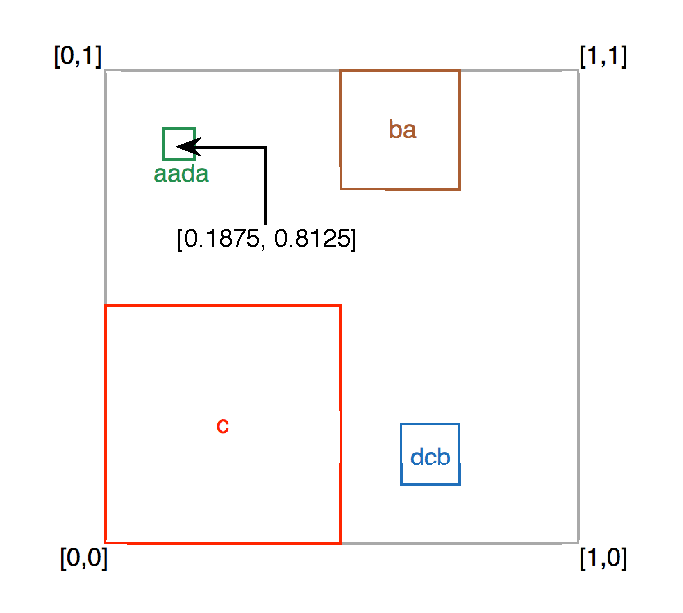
\includegraphics[width=80mm]{geohash.eps}
  \caption{Ukázka čtverců algoritmu Geohash v jednotkovém čtverci.}
  \label{fig:geohash}
\end{figure}

Nyní bychom chtěli algoritmus Geohash použít pro hledání podobných obrázků v Profimedia datasetu. Každému deskriptoru bychom nejprve přiřadily název. Množina podobných obrázků by pak obsahovala obrázky, které mají $Similarity$ s porovnávaným obrázkem nějak omezenou. Problémem je, že pomocí Geohash čtverců nedokážeme takovou oblat přesně definovat. Můžeme se ale pokusit co nejvíce oblast pomocí čtverců aproximovat. 

Pokud bychom chtěli použít Geohash pro hledání podobných vektorů přímo, narazili bychom na několik problémů. Například oblast s ohraničenou mírou $Simiarity$ nejde popsat přesně pomocí čtverců. Lze libovolně přesně aproximovat, ale s každou přesnější aproximací vzrůstá počet potřebných čtverců a zhoršuje se efektivita algoritmu. Obrázek \ref{fig:geohash_use} ukazuje jak bychom mohli použít Geohash algoritmus pro hledání podobných deskriptorů ve dvojrozměrné dimenzi. Na obrázku je popsána situace, kdy hledáme deskriptory, které mají od bodu $[0.5, 0.5]$ vzdálenost $0.5$. Tučně ohraničený čtverec vyznačuje hledanou oblast, $12$ čárkovaných čtverců tvoří aproximovanou oblast.

\begin{figure}[h]
  \centering
  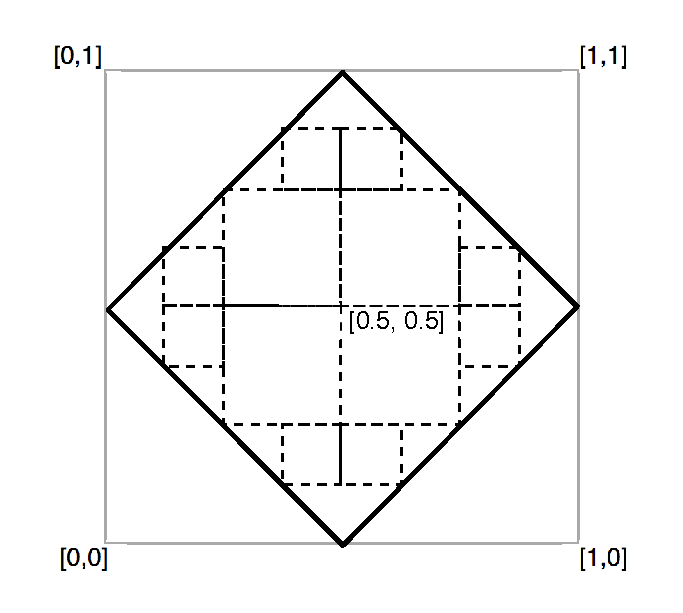
\includegraphics[width=80mm]{geohash_use.eps}
  \caption{Ukázka čtverců algoritmu Geohash v jednotkovém čtverci.}
  \label{fig:geohash_use}
\end{figure}

Ve dvou dimenzích by toto řešení fungovalo poměrně dobře. Deskriptory obrázků ovšem mají $4096$ složek a počet potřebných čtverců pro stejnou míru aproximace roste s každou dimenzí exponenciálně.

\section{Řešení}

Naše řešení využívá princip algoritmu Geohash. Jde nám o to, převést hledání podobných vektorů na fulltextové vyhledávání. Vektory reálných čísel převedeme na množinu slov oddělenou mezerami --- řetězec. Slova pochází z množiny $\{0, 1,… 4095\}$. Každé složce vektoru deskriptoru tedy odpovídá právě jedno slovo z množiny slov. Nyní přiřadíme každému deskriptoru nějakou nějakou podmnožinu slov. Způsob přiřazení je klíčovým faktorem algoritmu, který ovlivňuje jeho efektivitu. Základním způsobem je přiřadit vektoru slova, která odpovídají nenulovým vektorům. Na deskriptorech obrázků z datasetu Profimedie to znamená, že každý vektor bude mít přiřazeno zhruba 1500 slov. To je stále příliš mnoho slov pro efektivní fulltextové vyhledávání. Elasticsearch v základní konfiguraci ani neumožňuje vyhledávat s dotazy delšími než tisíc slov. Musíme tedy množinu slov dále zmenšit. Můžeme například místo nenulovosti zvýšit požadovanou mez velikosti složky vektoru.

V našem řešení používáme jinou metodu. Seřadíme složky vektorů podle velikosti a slova přiřadíme pouze $K$ složkám s nejvyšší hodnotou. Pro $K = 4$ pak každému obrázku přiřadíme řetězec, například $\mathrm{"}2013\ 432\ 1065\ 3433\mathrm{"}$. Při vyhledávání podobného obrázku nejprve získáme jeho deskriptor a jeho přiřazený řetězec. Pomocí řetězce najdeme fulltextovým vyhledáváním $L$ obrázků. Výsledky seřadíme podle podobnosti s hledaným obrázkem mírou $Similarity$ a vrátíme obrázky, které jsou v kategorii \uv{podobné}, nebo \uv{téměr shodné}. Pro správné fungování je nutné dobře nastavit hodnoty $K$ a $L$. Jejich zvýšení vede k větší přesnosti na úkor rychlosti algoritmu.

\section{Implementace}

Celá služba je implementována nezávisle na zbytku projektu. Jedná se o program \lstinline{similar_img_finder} napsaný v jazyce go. Jako databáze je použita Elasticsearch. Nejprve je nutné naimportovat data příkazem

\begin{lstlisting}
  similar_img_finder import -n 1000000 -e 9200 -k 500 -f data.gz
\end{lstlisting}

Parametr \lstinline{-n} určuje, kolik dat se má naimportovat, parametr \lstinline{-e} určuje na kterém portu běží Elasticsearch, parametr \lstinline{-k} odpovídá hodnotě $K$ a parametr \lstinline{-f} je cesta k souboru s importovanými daty.

Nyní můžeme spustit server na portu $8585$ příkazem

\begin{lstlisting}
  similar_img_finder server -p 8585 -l 100 -e 9200
\end{lstlisting}

Parametr \lstinline{-l} odpovídá hodnotě $L$.

Pokud chceme nyní získat id podobných obrázků k obrázku s id \uv{0000000003}, můžeme využít JSON HTTP API a získat výsledky na adrese \lstinline{localhost:8585/similar?id=0000000003}.





